\section{Pagerank}
\FloatBarrier\FloatBarrier
\begin{figure}[h]
	\centering
	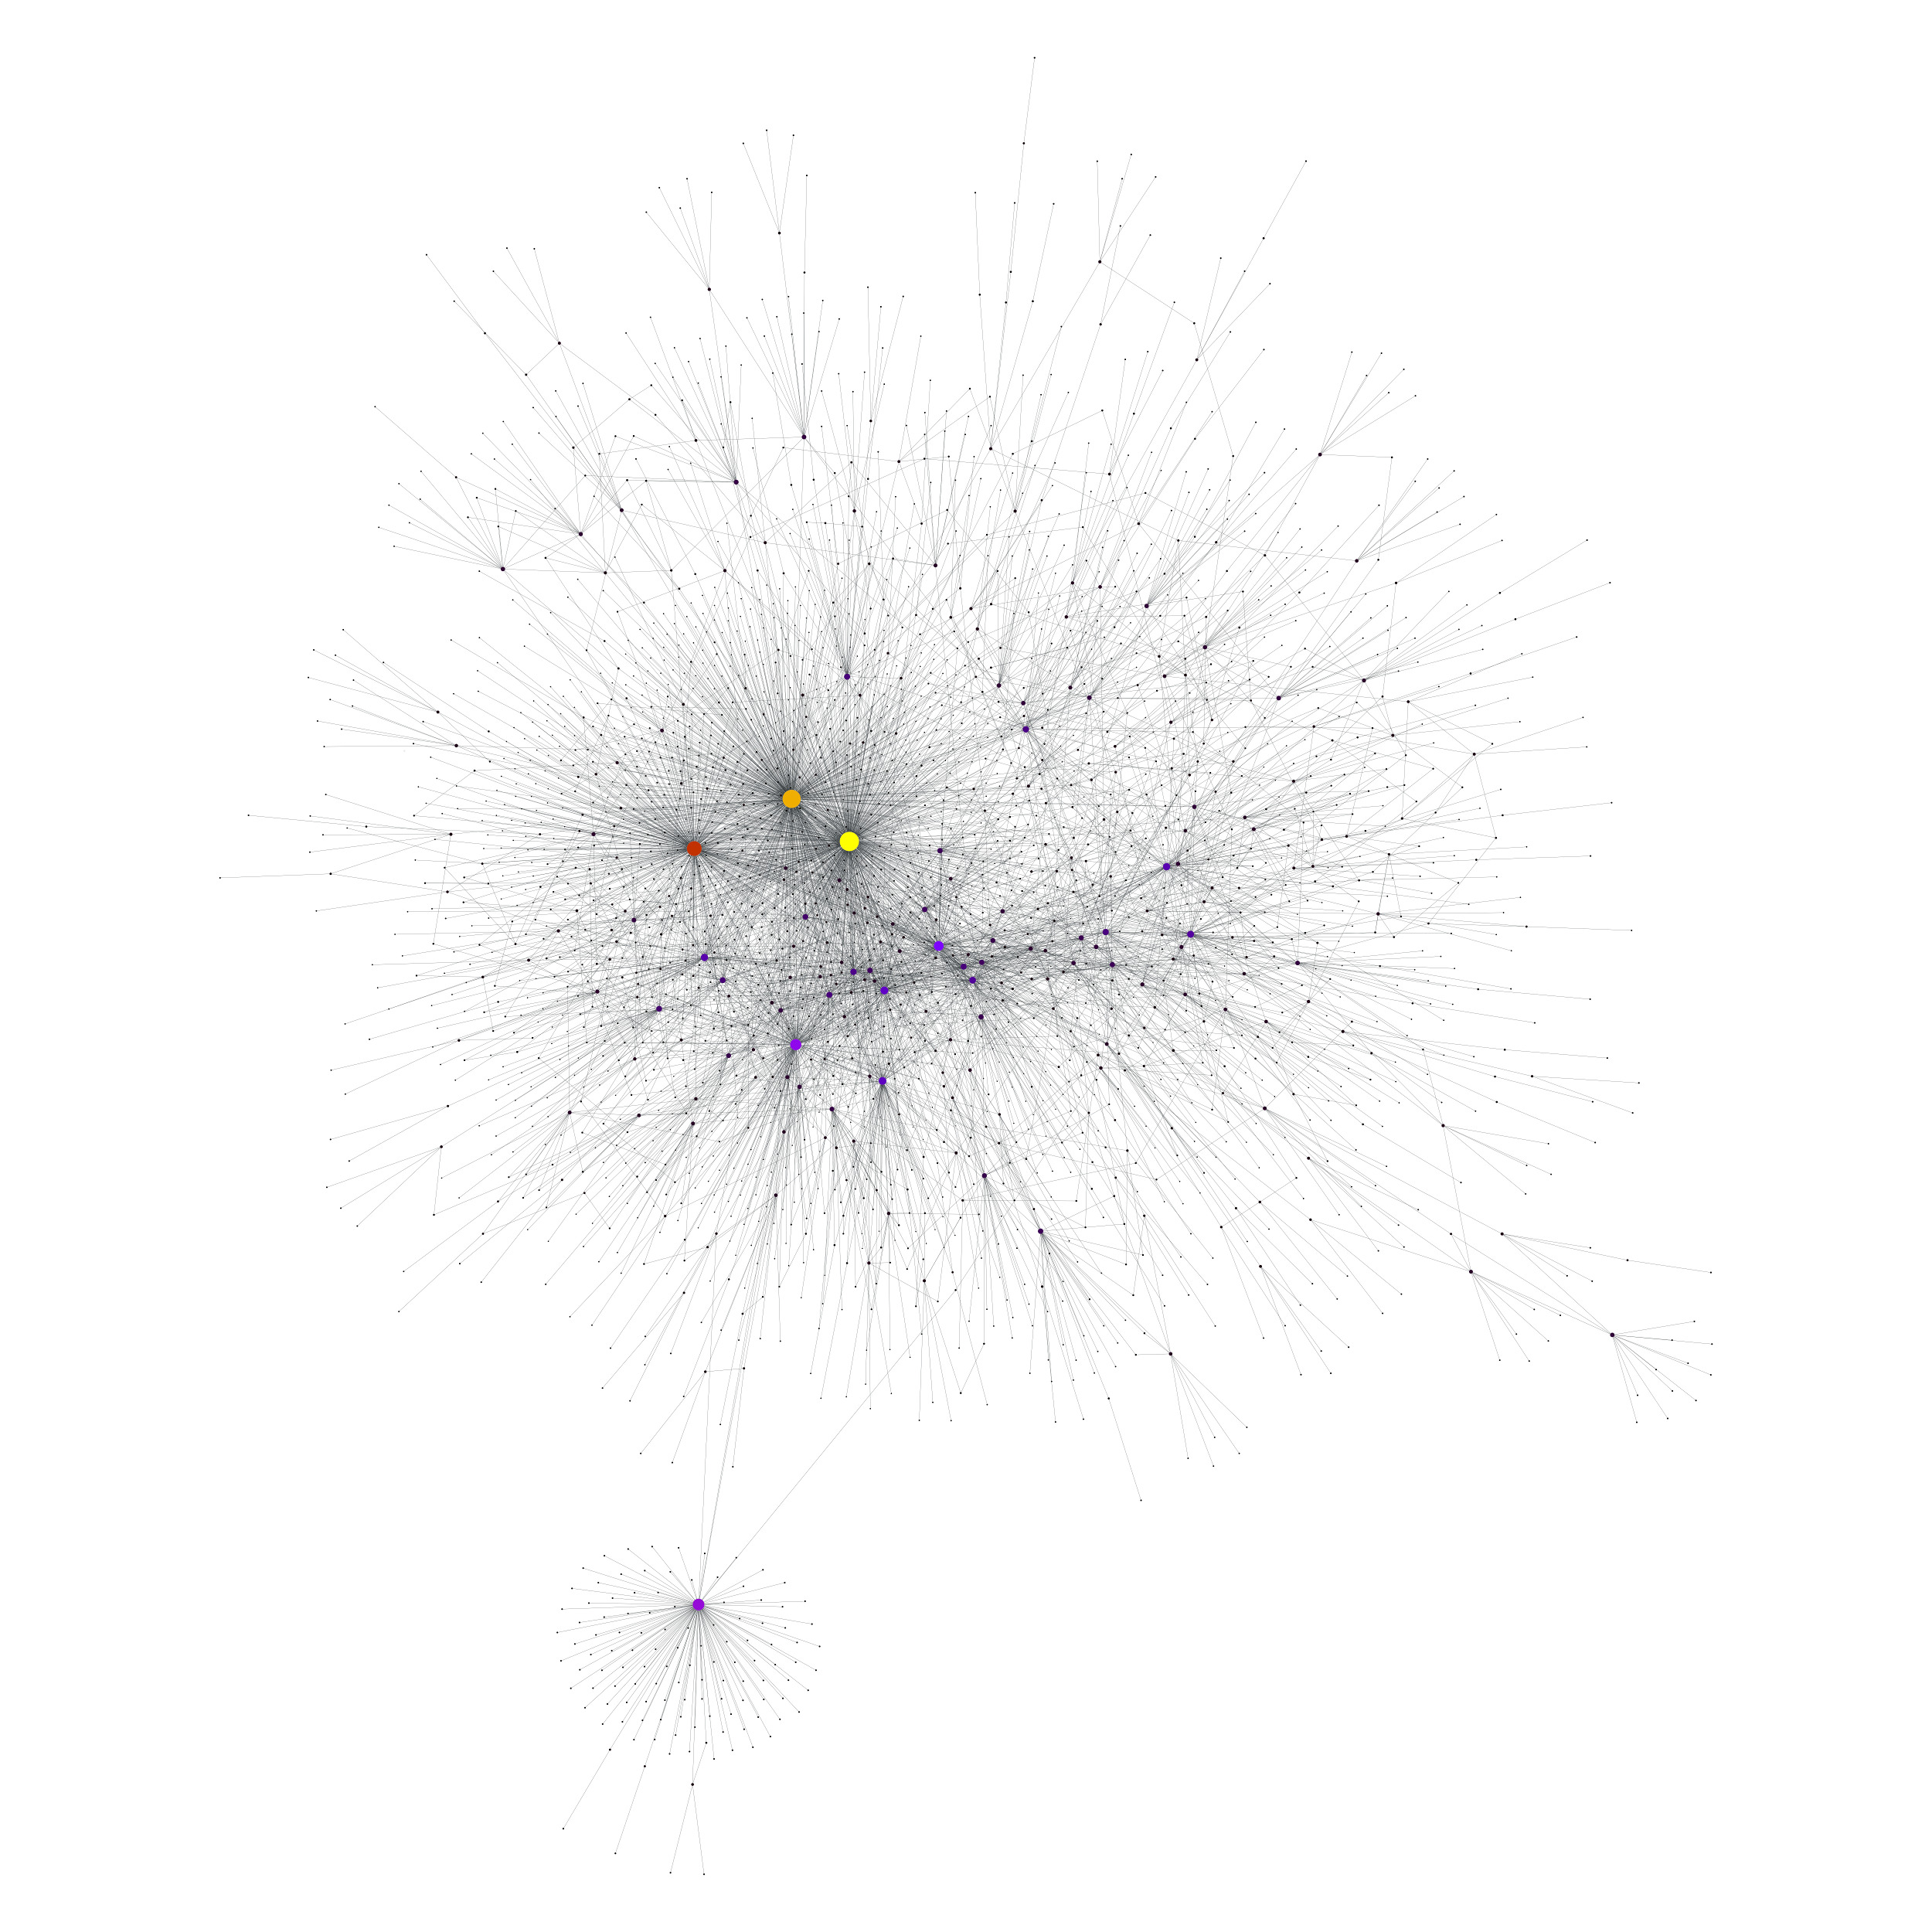
\includegraphics[width=\textwidth]{pagerank_8k}
	\caption{Działanie algorytmu pagerank na przykładowym grafie}
\end{figure}
\FloatBarrier
\begin{figure}[h]
	\centering
	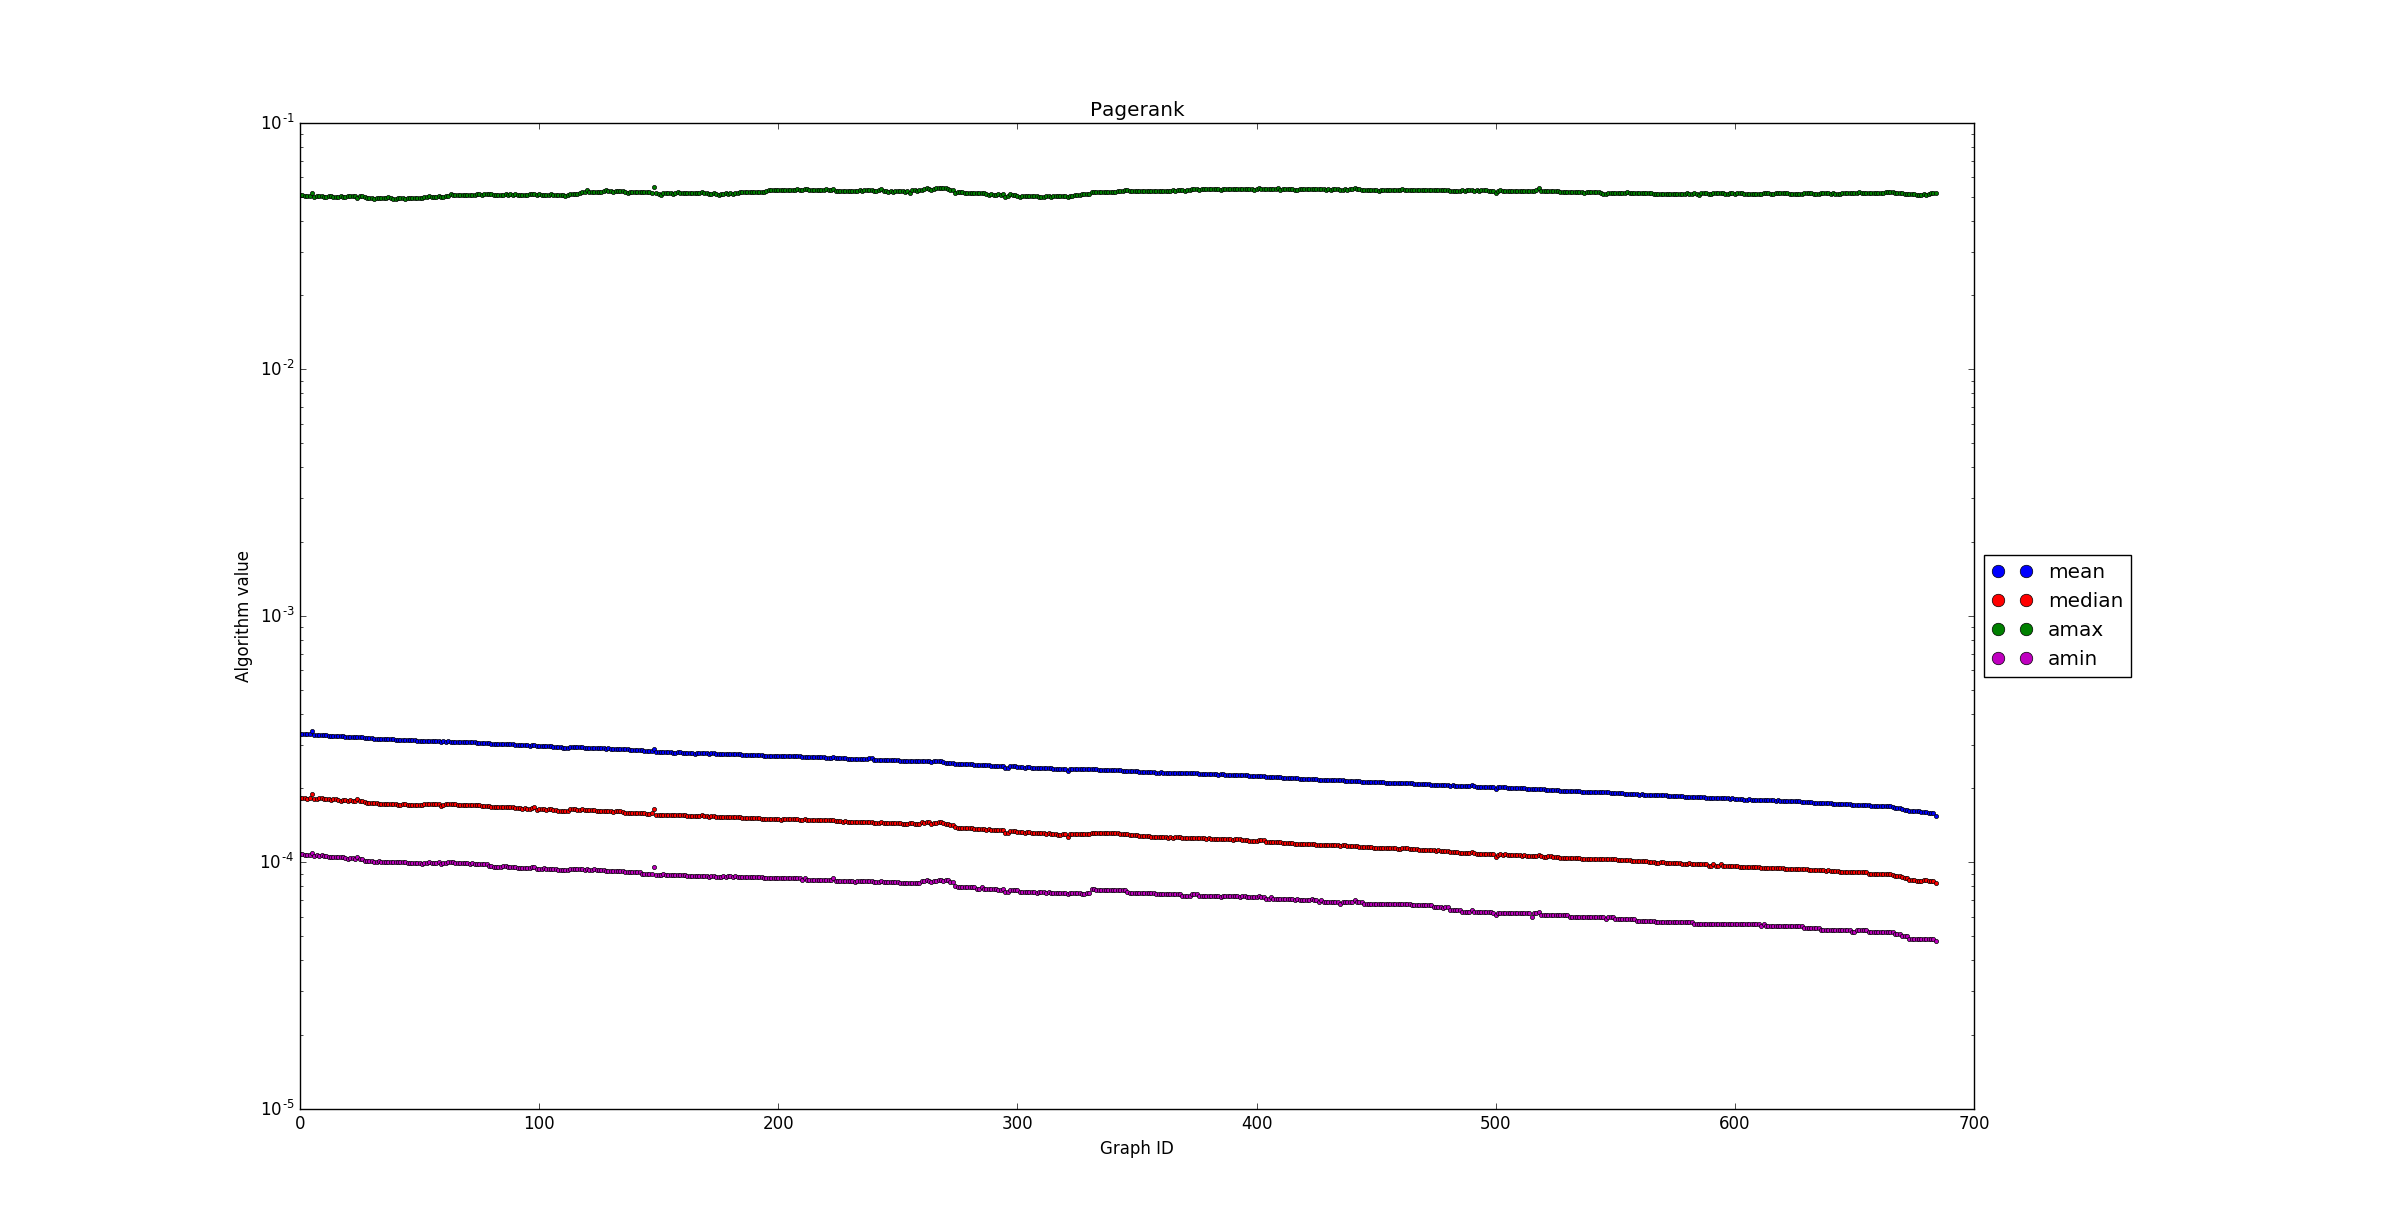
\includegraphics[width=\textwidth]{pagerank}
	\caption{Wyniki algorytmu pagerank}
\end{figure}
\FloatBarrier\FloatBarrier
\begin{figure}[h]
	\centering
	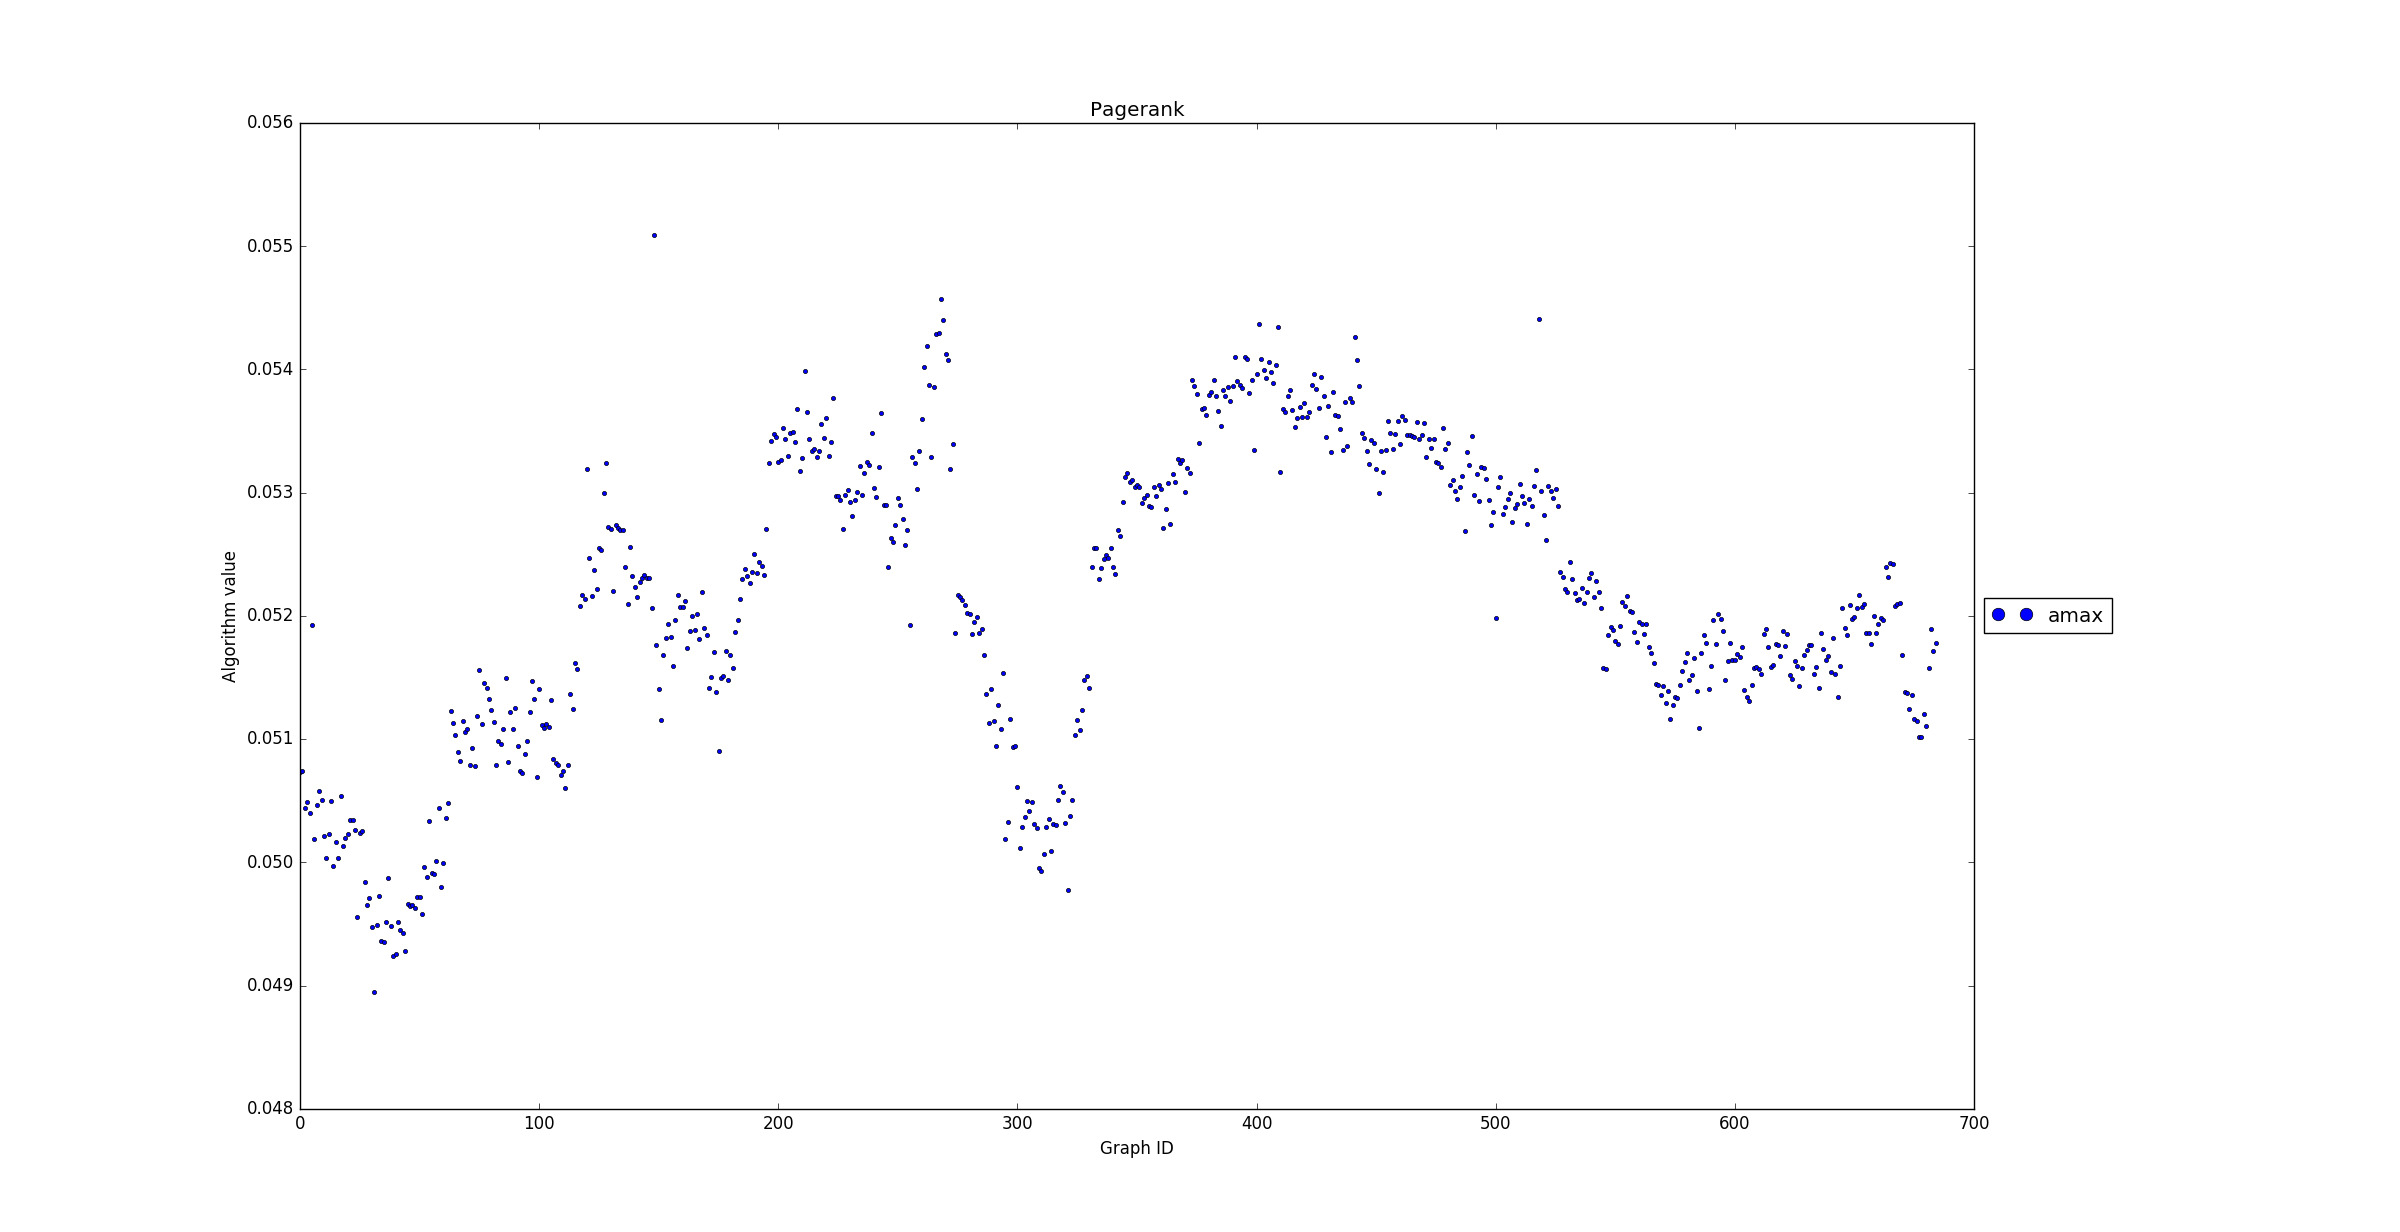
\includegraphics[width=\textwidth]{pagerank_max}
	\caption{Maksymalne wartości pagerank}
\end{figure}
\FloatBarrier\FloatBarrier
\begin{figure}[h]
	\centering
	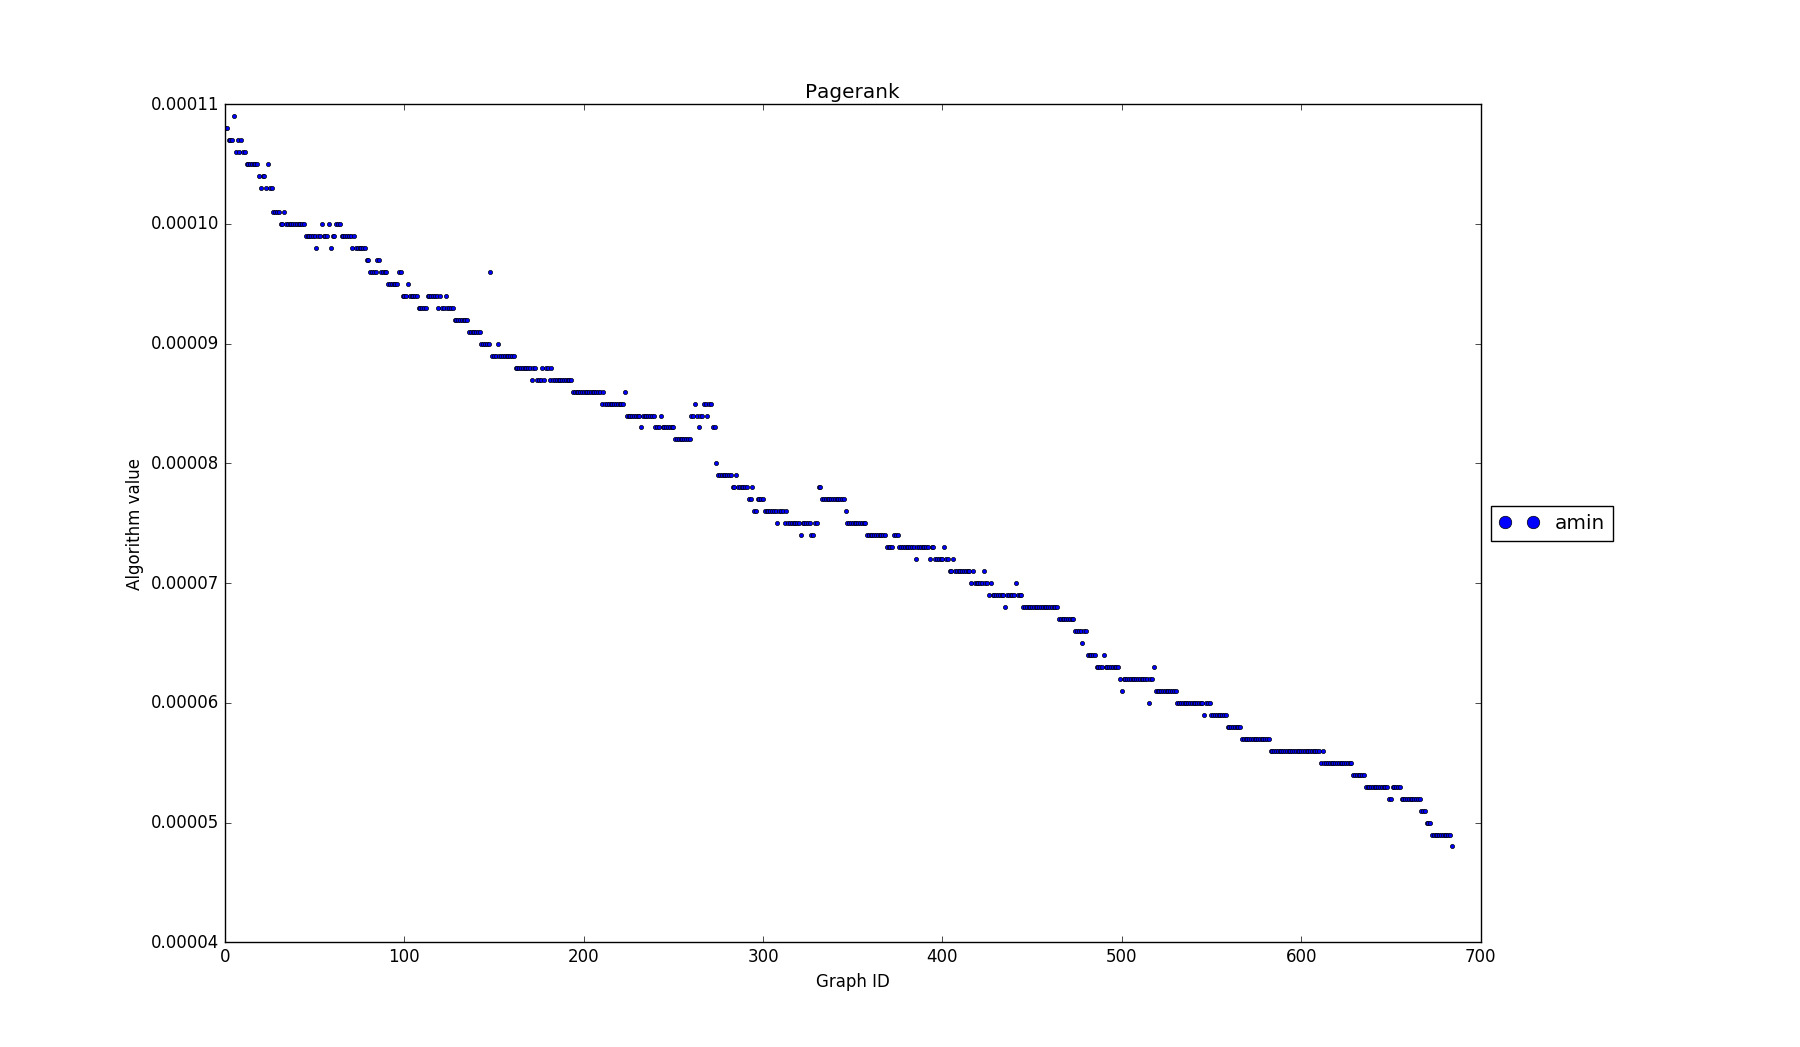
\includegraphics[width=\textwidth]{pagerank_min}
	\caption{Minimalne wartości pagerank}
\end{figure}
\FloatBarrier\FloatBarrier
\begin{figure}[h]
	\centering
	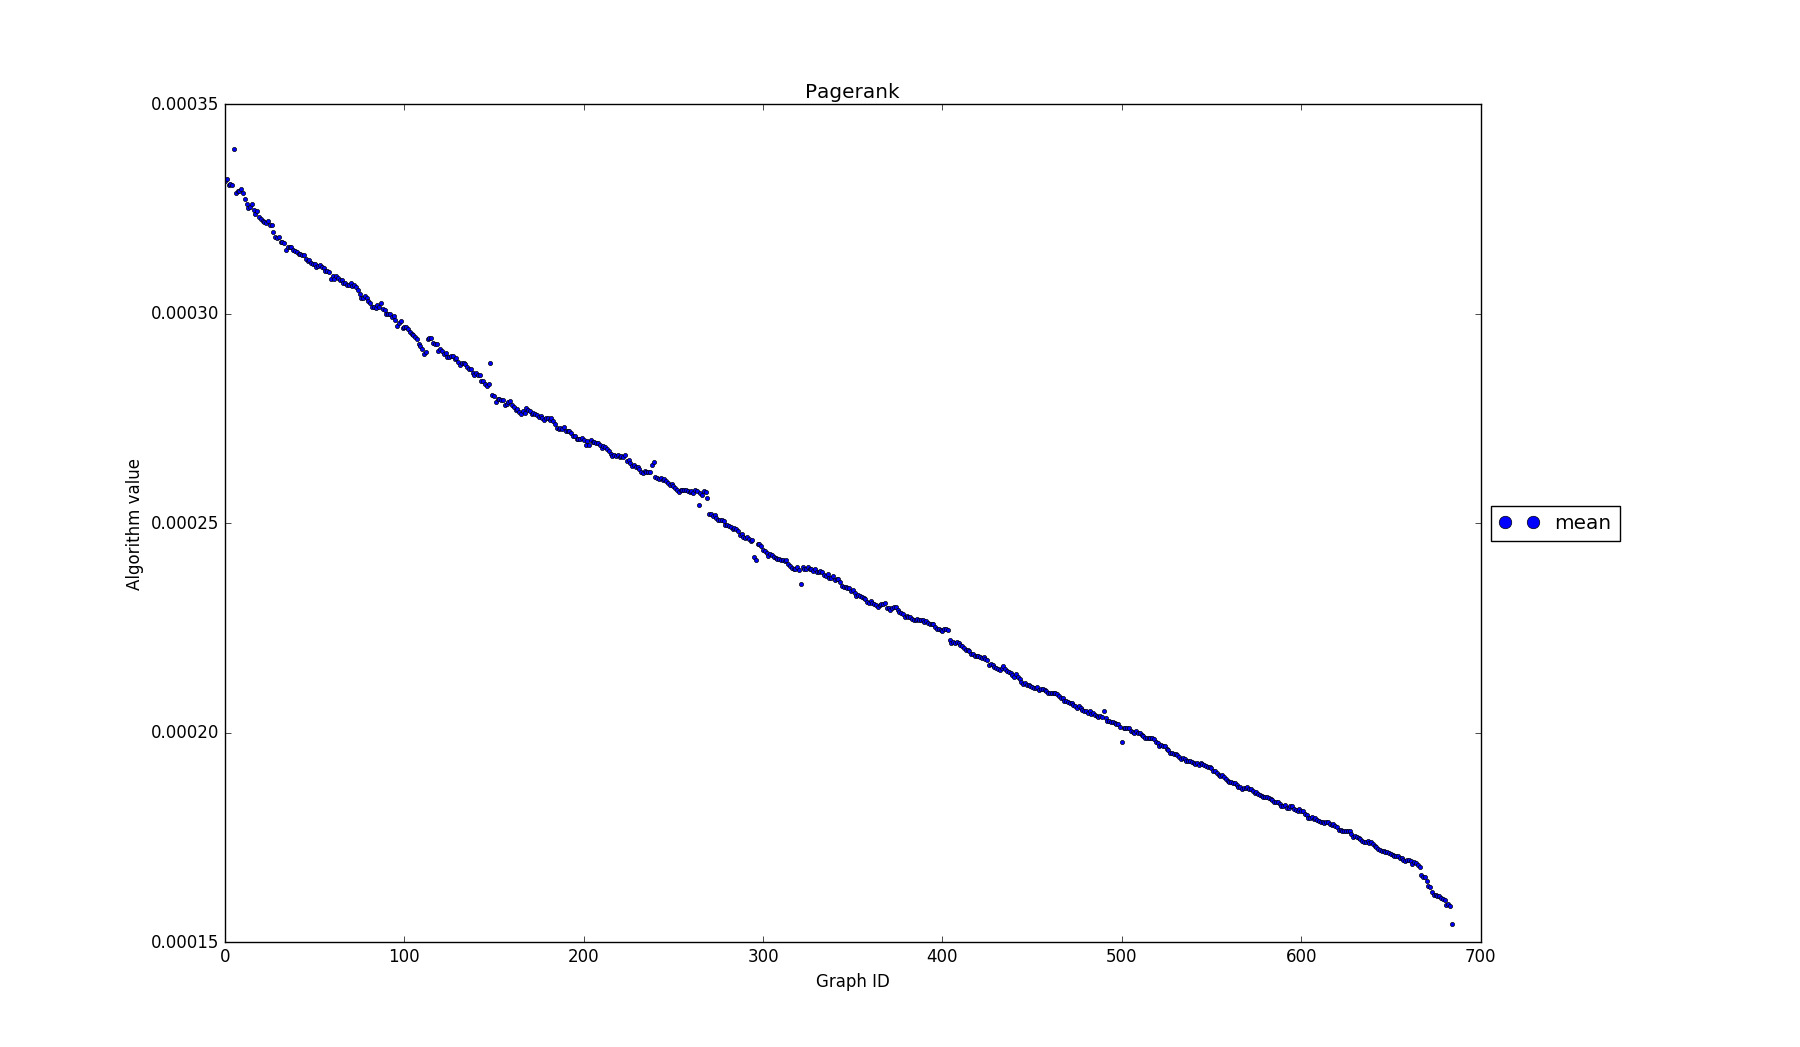
\includegraphics[width=\textwidth]{pagerank_mean}
	\caption{Średnie wartości pagerank}
\end{figure}
\FloatBarrier\FloatBarrier
\begin{figure}[h]
	\centering
	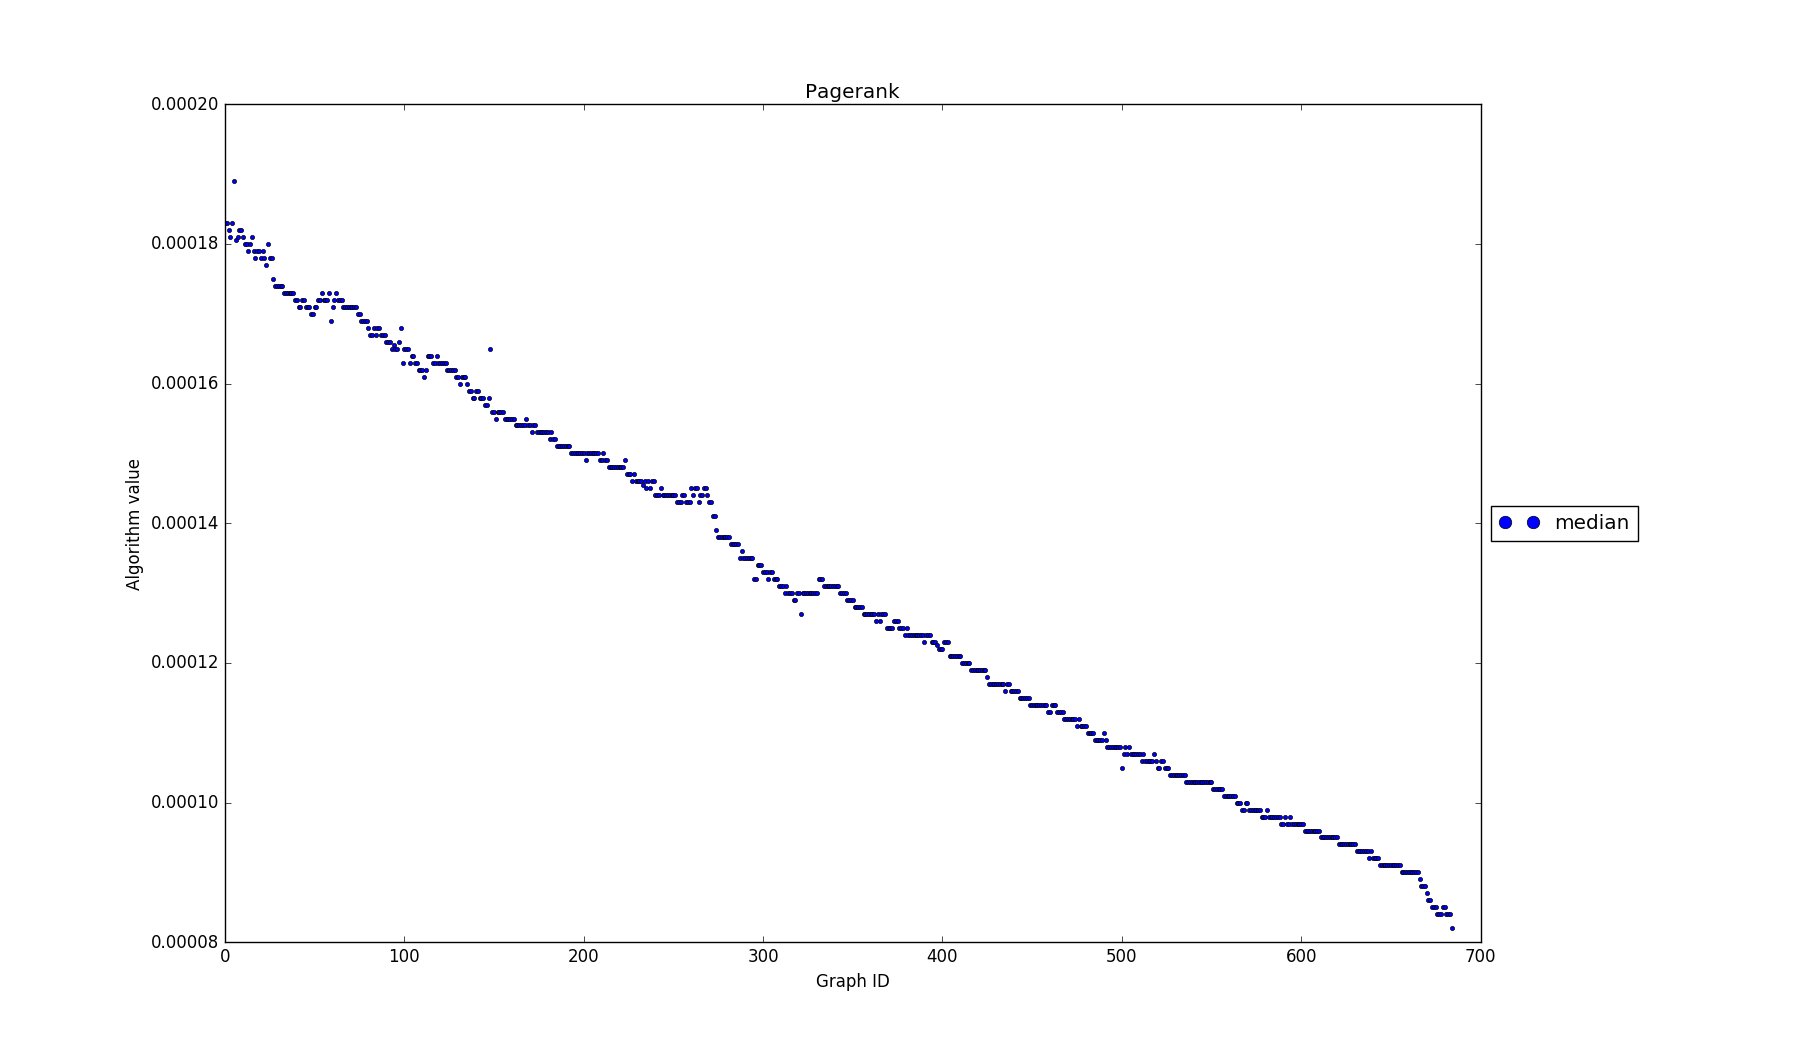
\includegraphics[width=\textwidth]{pagerank_median}
	\caption{Mediana wartości pagerank}
\end{figure}
Pagerank jest miarą tego jak dużo innych wierzchołków odwołuje się do badanego. Nie jest to równoznaczne ze stopniem wierzchołka ale ma on duży wpływ na wynik. W badanym okresie gęstość sieci malała, co daje się zauważyć również w spadku średniego wyniku algorytmu. Mimo tego maksymalna wartość pagerank, mimo drobnych fluktuacji, zachowuje podobny poziom. Wskazuje to na to, że nowe wierzchołki były w dużej mierze dodawane na obrzeżach a nie w środku sieci.
\FloatBarrier
\newpage